\chapter{Measuring the antenna response of SALSA by observing the Sun}

In this chapter we describe how you can measure the antenna response of SALSA by
observing the Sun. The Sun is a bright radio source and a small angular size compared
to the angular resolution of SALSA. By measuring the total power received
by the telescope at different angular separations from the Sun we get the
reponse function of the SALSA antenna. Note that in this project we are only
interested in measuring the relative response in different directions, i.e.
we do not require an absolute flux scale calibration of the antenna.

\section{When is a good time to observe?}
In this project we need the Sun to be up, i.e. it has to be daytime in Onsala.
To avoid disturbing radio emisson from the Earth itself it is good to observe
when the Sun is as high above the horizon as possible. This means that it is
good to observe around noon in Sweden, i.e. 11 UT, but also earlier or later
times are fine (in particular during the long Swedish summer days). To find out
exactly where the Sun is at a specific time you may use the free planetarium
software Stellarium. This software is described briefly in the \emph{SALSA user
manual} available via the SALSA website.

\section{Tracking positions relative to the Sun}
To observe the Sun we must know where to point the telescope at a given time.
Finding the celestial coordinates of the Sun can be tricky since it is not
stationary in the common Glactic or Equatorial coordinate systems (because of
the Earth's movement around the Sun). The SALSA control program can however
calculate the position of the Sun at any given time automatically. To
track the Sun, select \emph{The Sun} as desired target (instead of the default
\emph{Galactic}) in the control program. The program will now automatically
calculate where the Sun is right now. 

However, to measure the antenna response it is not enough to measure on the Sun
itself, we also want to measure at different angular separations relative to
the Sun. Conveniently, the SALSA control program can also automatically track
positions relative to the Sun by specifying local horizontal (altitude,
azimuth) offsets. For example, to track a point on the sky which is always
3 degrees offset in azimuth angle from the Sun, chose the Sun as the target
and enter an azimuth offset of 3 in the control program, then press the
button \emph{Track}. To switch to another relative position you
have to first press \emph{Stop} to be able to input new offets, and then
track the new position.

\section{Measuring total power from the Sun}
The SALSA control program, as described in the \emph{SALSA user manual}, was
developed to measure radio emission from neutral hydrogen. When observing
hydrogen it is crucial to find out how the emission changes with different
frequencies close to 1420\,MHz, and therfore the program was developed
primarily to measure {spectra}, i.e. a plot of the radio emission as a function
of frequency within a specific frequency range. However, when observing the Sun
to measure the antenna response function, we are only interested in the total
power received by the antenna in some frequency range.

%Since the SALSA receiver works best around 1420\,MHz we chose a nearby
%frequency such as 1410\,MHz as center frequency for our observations. This is
%done in the tab \emph{Advanced} in the \emph{Receiver control} part of the
%control program.  The default bandwidth does not need to be changed.

Since the SALSA receiver works best around 1420\,MHz we will observe the Sun at
this or a nearby frequency. To be sure not to include any hydrogen emission
from the galaxy (which may be in the background of the Sun) we chose 1410\,MHz
as center frequency for our observations. This is done in the tab
\emph{Advanced} in the \emph{Receiver control} part of the control program.
This frequency is close enough for the receiver to work well, but far enough
from 1420\,MHz to not include any emission from galactic hydrogen.  The default
bandwidth does not need to be changed.

By default, the program will observe in \emph{Switched} mode, which is used for
spectral line observations of hydrogen. This mode removes disturbances from
the receiver on the signal, but will also remove much of the total power 
received from the final spectrum. Since we want the total
power, we need to change the mode of SALSA from \emph{Switched} to
\emph{Signal}, also in the tab \emph{Advanced} in the \emph{Receiver control}
part.

Once we have specified the frequency and the signal-mode we are ready to
measure.  Make sure you are tracking a desired position relative to the Sun
(using offsets) and press \emph{Measure}. The default integration time of 10
seconds is enough to detect the Sun, it is very bright also in radio emission.

When the measurement has finished we need to extract the total power measured.
This is done by lookin in the terminal you used to start SALSA. After your 
measurement has finished you will see output similar to the line 
\begin{verbatim}
SPECTRUM INFO: Offset_alt=0.0 deg. Offset_az=1.5 deg. Total power = 670.0
\end{verbatim}
assuming you selected an azimutal offset of 1.5 degrees relative to the Sun.

Note the offset numbers and the total power measured, for example 
in a spreadsheet (e.g. using the free software Libre Office Calc available 
via www.libreoffice.org).

\section{Plotting the antenna response function}
Using your measurements you may now plot the antenna response function
relative to the Sun. If you plot the total power as a function
of azimutal offset, it should look similar to Fig. \ref{fig:beam}.

\begin{figure}[ht]
\begin{center}
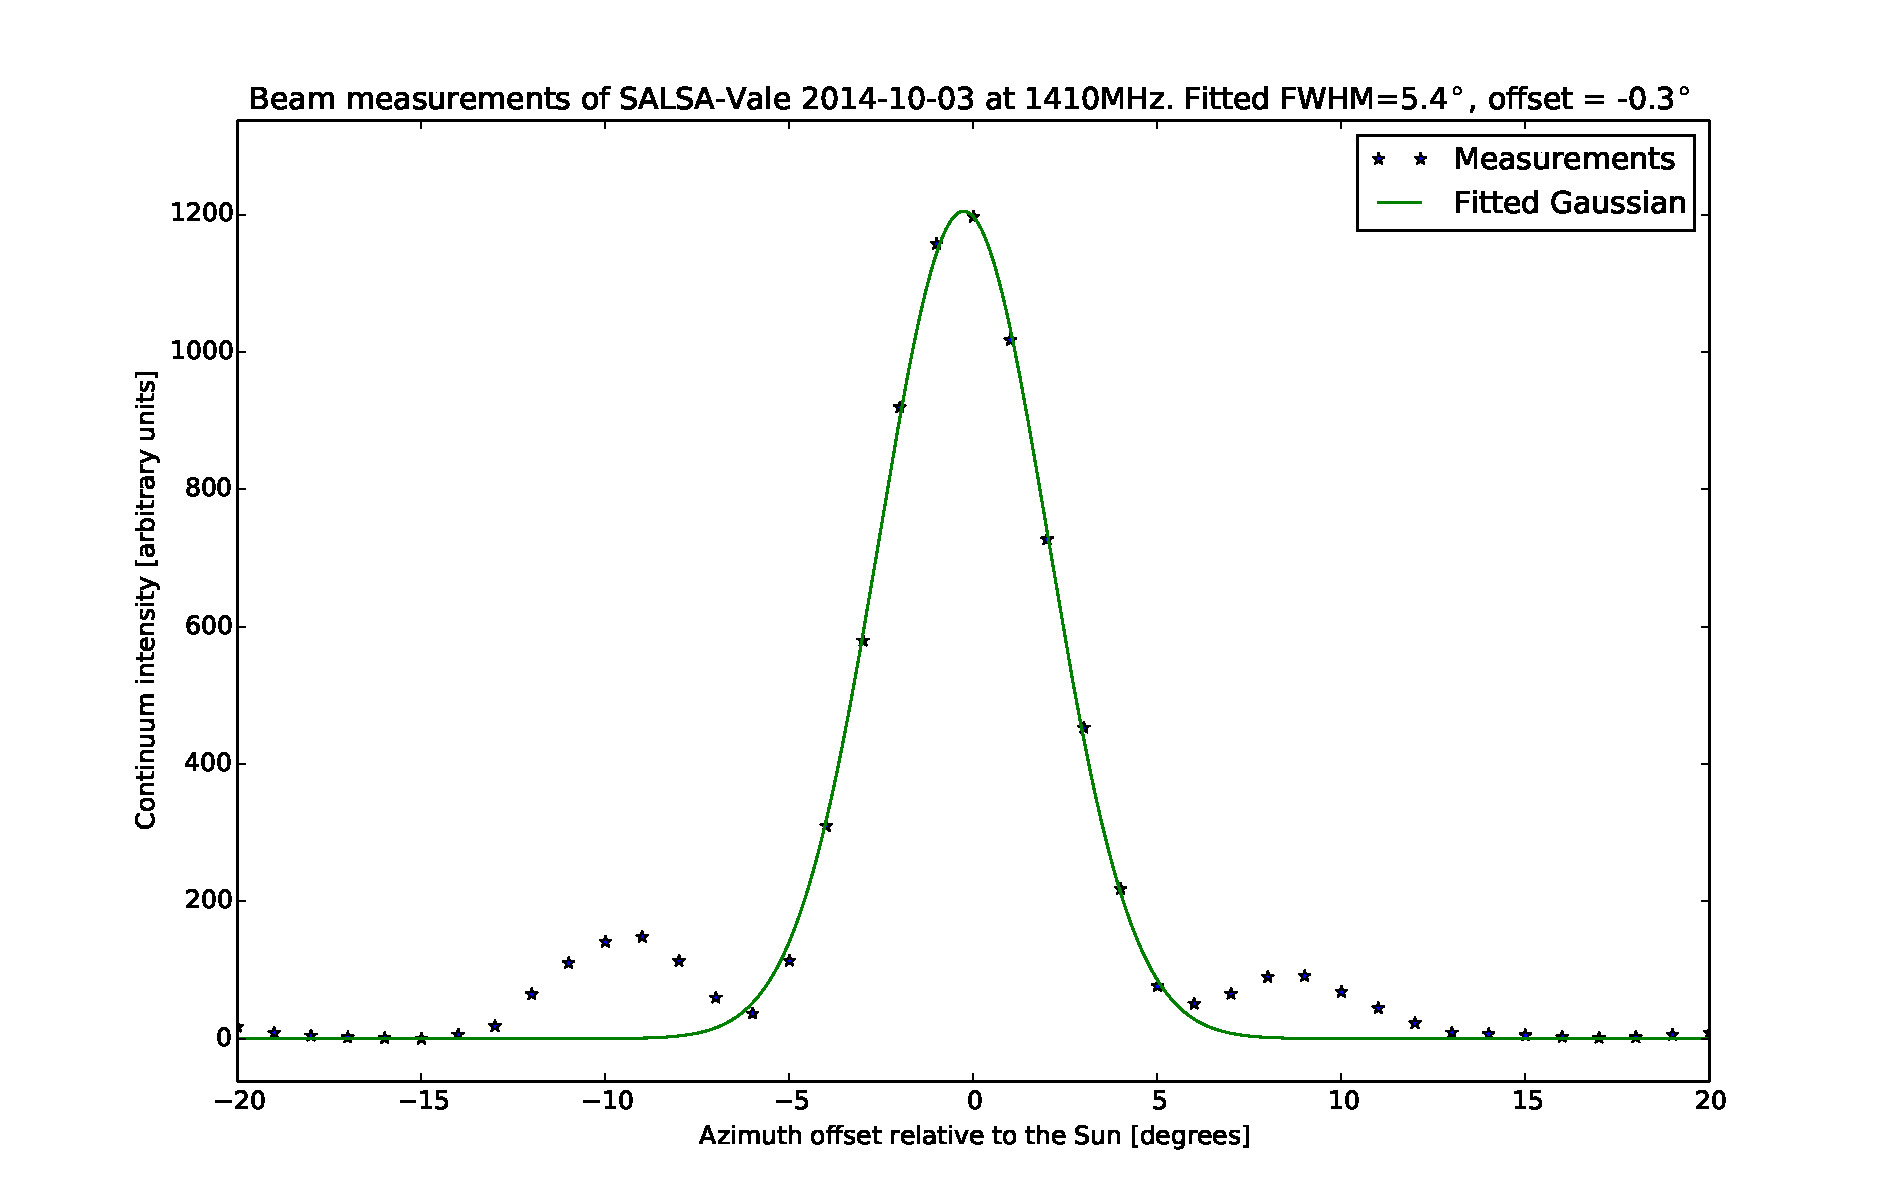
\includegraphics[width=\textwidth]{../figures/Beam_vale_2014-10-03.pdf}
\end{center}
\caption{The beam of Vale measured using the Sun at 1410\,MHz. A Gaussian fit
gives the FWHM=5.4$^\circ$. The sidelobes of the Sinc-function are clearly
visible, as expected for a circular aperture.}
\label{fig:beam}
\end{figure}

